\begin{figure*}[t]
\centering
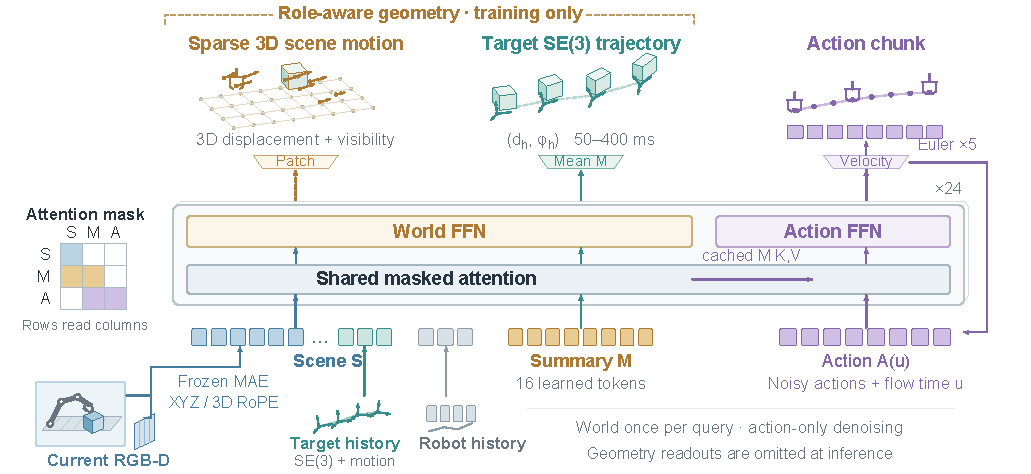
\includegraphics[width=\textwidth]{figures/Fig2/fig2_se3wam.pdf}
\caption{\textbf{Overview of \ours.}
(a) Architecture. The current RGB-D frame and the target and robot histories form scene tokens $S$, alongside summary tokens $M$ and noisy action tokens $A$. All tokens share masked attention, followed by separate world and action FFNs. The sparse 3D flow and the target SE(3) trajectory are predicted from $S$ and $M$.
(b) Attention mask. Rows are queries and columns are keys. Hatched cells are masked.
(c) Training and inference. The world and action streams are trained jointly. At inference, the world stream runs once and the prediction heads are skipped.}
\label{fig:architecture}
\end{figure*}
